\documentclass{minimal}

\usepackage{tikz}
\usetikzlibrary{plotmarks}

% Load the library
\usetikzlibrary{external}

% Activate it
\tikzexternalize

\usepackage{ucs}
\usepackage[utf8x]{inputenc}
%\usepackage{babel}
\usepackage{fontenc}
\usepackage{graphicx}


\usepackage{pgfplots}
\pgfplotsset{compat=1.9}
%\PrerenderUnicode{±}

\begin{document}

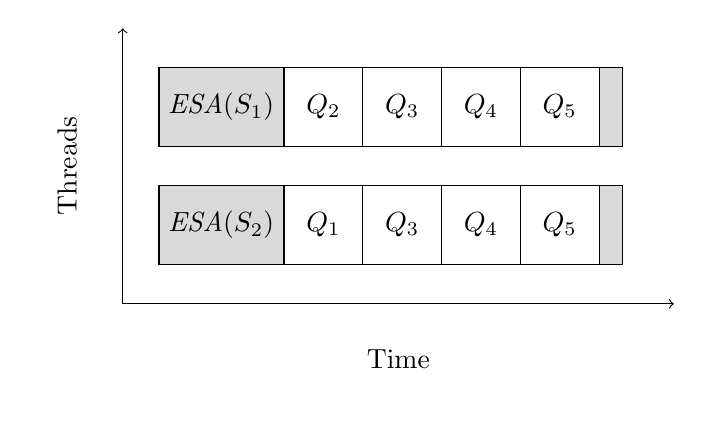
\begin{tikzpicture}[
		every node/.style={
			rectangle,
			draw,
			minimum height=1cm,
			minimum width=1cm
		},
		derp/.style={
			draw=black,
			fill=black!15
		}]


		\draw[->] (0,0) -- coordinate (x axis mid) (7,0);
		\draw[->] (0,0) -- coordinate (y axis mid) (0,3.5);

		%labels
		\node[draw=none,below=0.2cm] at (x axis mid) {Time};
		\node[draw=none,rotate=90, above=0.2cm] at (y axis mid) {Threads};

		\node[derp] at (1.25,2.5) (a1) {$\mathit{ESA}(S_1)$};
		\node[right of=a1, node distance=1.3cm] (a2) {$Q_2$};
		\node[right of=a2] (a3) {$Q_3$};
		\node[right of=a3] (a4) {$Q_4$};
		\node[right of=a4] (a5) {$Q_5$};
		\node[right of=a5, minimum width=0.3cm, node distance=0.65cm, derp] (a6) {};

		\node[below of=a1, node distance=1.5cm, derp] (b1) {$\mathit{ESA}(S_2)$};
		\node[right of=b1, node distance=1.3cm] (b2) {$Q_1$};
		\node[right of=b2] (b3) {$Q_3$};
		\node[right of=b3] (b4) {$Q_4$};
		\node[right of=b4] (b5) {$Q_5$};
		\node[right of=b5, minimum width=0.3cm, node distance=0.65cm, derp] (b6) {};

	\end{tikzpicture}

	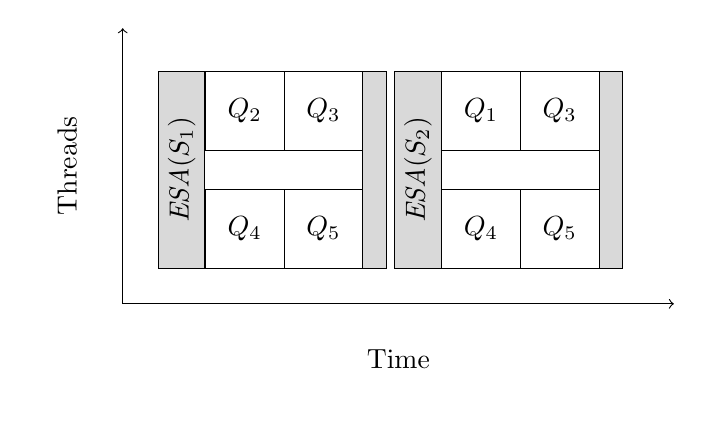
\begin{tikzpicture}[
		every node/.style={
			rectangle,
			draw,
			minimum height=1cm,
			minimum width=1cm
		},
		derp/.style={
			draw=black,
			fill=black!15,
			minimum height=2.5cm
		}]


		\draw[->] (0,0) -- coordinate (x axis mid) (7,0);
		\draw[->] (0,0) -- coordinate (y axis mid) (0,3.5);

		%labels
		\node[draw=none,below=0.2cm] at (x axis mid) {Time};
		\node[draw=none,rotate=90, above=0.2cm] at (y axis mid) {Threads};

		\node[rotate=90,
			minimum width=2.5cm,
			draw=black,
			fill=black!15,
			minimum height=0.4cm] at (0.75,1.7) (a1) {$\mathit{ESA}(S_1)$};

		\node[right of=a1,draw=none,node distance=0.80cm] (helper) {};

		\node[above of=helper, node distance=0.75cm] (a2) {$Q_2$};
		\node[right of=a2] (a3) {$Q_3$};
		\node[below of=helper, node distance=0.75cm] (a4) {$Q_4$};
		\node[right of=a4] (a5) {$Q_5$};
		\node[right of=helper, minimum width=0.3cm, node distance=1.65cm, derp] (a6) {};

		\node[rotate=90,
			minimum width=2.5cm,
			draw=black,
			fill=black!15,
			minimum height=0.4cm] at (3.75,1.7) (b1) {$\mathit{ESA}(S_2)$};

		\node[right of=b1,draw=none,node distance=0.80cm] (helper2) {};

		\node[above of=helper2, node distance=0.75cm] (b2) {$Q_1$};
		\node[right of=b2] (b3) {$Q_3$};
		\node[below of=helper2, node distance=0.75cm] (b4) {$Q_4$};
		\node[right of=b4] (b5) {$Q_5$};
		\node[right of=helper2, minimum width=0.3cm, node distance=1.65cm, derp] (b6) {};

	\end{tikzpicture}

\end{document}
